\chapter[Classical SR Quantities]{Classical quantities in Special Relativity}
\section{4-velocity}
In classical mechanics the velocity of a particle is:
\begin{equation}
  \vec{u} = \dv{\vec{r}}{t}
\end{equation}
This still holds in Relativity, but only for the spatial coordinates, so we must choose something that is invariant to define the 4-velocity tensor.
We know that $\diff{s}^2$ is invariant so let's introduce another invariant quantity based on this:
\begin{equation}
  \diff{\tau}^2 = \dfrac{\diff{s}^2}{c^2}
\end{equation}
First we can notice that $\sqbr{\diff{\tau}} = \sqbr{s}$ and if we expand $\diff{\tau}^2$ from its definition:
\begin{equation}
  \begin{split}
    \diff{\tau}^2 &= \diff{t}^2 - \dfrac{\norm{\diff{\vec{r}}}^2}{c^2} =\\[8pt]
    &= \diff{t}^2 \brackets{1 - \dfrac{u^2}{c^2}} = \dfrac{\diff{t}^2}{\gamma^2(u)}
  \end{split}
\end{equation}
So $\diff{\tau} = \dfrac{\diff{t}}{\gamma(u)}$. If we choose the IRF of istantaneous rest, also called \textbf{co-moving IRF} we have that $\diff{\tau}$ is:
\begin{equation}
  \diff{\tau} = \dfrac{\diff{t}}{\gamma(0)} = \diff{t}
\end{equation}
Thus, $\diff{\tau}$ is the $\diff{t}$ evaluated in the IRF in which the particle is at rest and is the proper time interval.\\
Let's go back to our original problem and define the 4-velocity tensor as:
\begin{equation}
  u^{\mu} = \dv{x^{\mu}}{\tau}
\end{equation}
The tensor $u^{\mu}$ is contravariant. Now, by applying the chain rule we get:
\begin{equation}
  u^{\mu} = \dv{x^{\mu}}{\tau} = \dv{x^{\mu}}{t} \dv{t}{\tau} =\gamma(u) \dv{x^{\mu}}{t}
\end{equation}
Now we exploit the definiton of $\diff{x}^{\mu} = \brackets{c\diff{t}, \diff{\vec{r}}}$ leading to:
\begin{equation}
  \boxed{u^{\mu} = \gamma(u) \brackets{c, \vec{u}}}
\end{equation}
Now we should ask ourselves what the magnitude of the 4-velocity is. By using the definition of magnitude we have established we get:
\begin{equation}
  u^2 = u^{\mu}u_{\mu} = \gamma^2(u)\brackets{c^2 - u^2} = \cancel{\gamma^2(u)}c^2\cancel{\brackets{1 - \dfrac{u^2}{c^2}}} = c^2
\end{equation}
So the magnitude of the 4-velocity will always be $c$. Even for an object at rest we have:
\begin{equation}
  u^{\mu} = \gamma(u)\brackets{c, \vec{u}} = \gamma(0)\brackets{c, \vec{0}} = \brackets{c, \vec{0}}
\end{equation}
And so the magnitude is indeed $c$. Now let us see what happens if we apply a Lorentz transformation to $\tensor{u}{^\mu} \rightarrow \tensor{u}{^\prime^\mu} = \tensor{\lm}{^\mu_\nu}\tensor{u}{^\nu}$:
\begin{equation}
  \tensor{u}{^\prime^\mu} =
  \begin{cases}
    \tensor{u}{^\prime^0} = \gamma \left( u^{0} - \dfrac{v}{c} u^{1} \right) \\[8pt]
    \tensor{u}{^\prime^1} = \gamma \left( u^{1} -  \dfrac{v}{c} u^{0}\right) \\[8pt]
    \tensor{u}{^\prime^2} = u^{2} \\[8pt]
    \tensor{u}{^\prime^3} = u^{3}
  \end{cases} =
  \begin{cases}
    \tensor{u}{^\prime^0} = \gamma \left( \gamma(u)c - \dfrac{v}{c} \gamma(u)u_x \right) \\[8pt]
    \tensor{u}{^\prime^1} = \gamma \left( \gamma(u)u_x -  \dfrac{v}{c} \gamma(u)c \right) \\[8pt]
    \tensor{u}{^\prime^2} = u^{2} \\[8pt]
    \tensor{u}{^\prime^3} = u^{3}
  \end{cases}
\end{equation}
After some calculations the first transformation leads to:
\begin{equation} \label{gamma_transformation}
  \dfrac{\gamma(u')}{\gamma(u)} = \gamma(v)\brackets{1-\dfrac{v u_x}{c^2}}
\end{equation}
From the second we get:
\begin{equation}
  \dfrac{\gamma(u')}{\gamma(u)}\tensor{u}{^\prime_x} = \gamma(v)\brackets{u_x - v}
\end{equation}
And so putting those equations together we have:
\begin{equation}
  \begin{split}
    \cancel{\gamma(v)}\brackets{1-\dfrac{v u_x}{c^2}}\tensor{u}{^\prime_x} = \cancel{\gamma(v)}\brackets{u_x - v} \\[8pt]
    \tensor{u}{^\prime_x} = \dfrac{u_x - v}{1-\dfrac{v u_x}{c^2}}
  \end{split}
\end{equation}
And we aslo obtain the relation:
\begin{equation}
  \gamma(u') = \dfrac{\gamma(u)\gamma(v)\brackets{u_x-v}}{\tensor{u}{^\prime_x}}
\end{equation}
Now the third transformation is simply:
\begin{equation}
  \gamma(u')\tensor{u}{^\prime_y} = \gamma(u)\tensor{u}{_y}
\end{equation}
Substituting the relation for $\gamma(u')$ gives:
\begin{equation}
  \begin{split}
    \dfrac{\cancel{\gamma(u)}\gamma(v)\brackets{u_x-v}}{\tensor{u}{^\prime_x}}\tensor{u}{^\prime_y} = \cancel{\gamma(u)}\tensor{u}{_y} \\[8pt]
    \tensor{u}{^\prime_y} = \dfrac{\tensor{u}{^\prime_x} \tensor{u}{_y}\sqrt{1-\dfrac{v^2}{c^2}}}{u_x-v}
  \end{split}
\end{equation}
\section{4-acceleration}
Similarly to what we did for the velocity we want to define a tensor for the acceleration. We define:
\begin{equation}
  a^{\mu} = \dv{u^{\mu}}{\tau} = \dv{u^{\mu}}{t}\dv{t}{\tau} = \gamma(u)\dv{u^{\mu}}{t}
\end{equation}
And so we have:
\begin{equation}
  \begin{split}
    a^{\mu} &= \gamma(u)\brackets{\dv{\brackets{\gamma(u)c}}{t}, \dv{\brackets{\gamma(u)\vec{u}}}{t}} = \\[8pt]
    &= \gamma(u)\brackets{c\dot{\gamma}(u), \dot{\gamma}(u)\vec{u} + \gamma(u)\vec{a}}
  \end{split}
\end{equation}
We can notice that the 4-acceleration $a^{\mu}$ is zero if and only if the vectorial acceleration $\vec{a}$ is zero. In fact if $u$ is constant:
\begin{equation}
  a^{\mu} = \gamma^2(u)\brackets{0,\vec{a}}
\end{equation}
In the co-moving IRF we additionally have that $\gamma(0) = 1$:
\begin{equation}
  a^{\mu} = \brackets{0,\vec{a}}
\end{equation}
Is the relation of orthogonality conserved for the 4-acceleration and the 4-velocity? The answer is yes and it can be shown knowing that the magnitude of any 4-velocity is constant and equal to $c$:
\begin{equation}
  \dv{c^2}{t} = 0 \implies \dv{\brackets{u^{\mu}u_{\mu}}}{t} = 0
\end{equation}
But if we perform the derivative:
\begin{equation}
  \begin{split}
    \dot{u}^{\mu}u_{\mu} + u^{\mu}\dot{u}_{\mu} = 0 \\[8pt]
    \dot{u}^{\mu}u_{\mu} + u_{\mu}\dot{u}^{\mu} = 0 \\[8pt]
    \boxed{a^{\mu}u_{\mu} = 0}
  \end{split}
\end{equation}
Notice that we raised and lowered an index in the second term of the expression and so this does not change any sign.\\
The square magnitude of $a^{\mu}$ is:
\begin{equation}
  a_{\mu}a^{\mu} = \begin{pNiceMatrix}
    0 & \vec{a}
  \end{pNiceMatrix}
  \begin{pNiceMatrix}
    0 \\ -\vec{a}
  \end{pNiceMatrix} = -a^2
\end{equation}
So the 4-velocity is a spacelike vector, instead the 4-acceleration is a timelike vector.\\
After defining the 4-velocity and the 4-acceleration we are ready to start talkin about dynamics in Special Relativity. In classical mechanics we have some fundamental principles:
\begin{itemize}
  \item Newton's \nth{1} law: Inertia
  \item Newton's \nth{2} law: $\sum \vec{F} = m\vec{a}$
  \item Newton's \nth{3} law
  \item Conservation laws
\end{itemize}
Inertia still holds in general relativity, but the Newton's \nth{2} law must not be true since we have a limit to the speed that a moving object can reach. Also Newton's \nth{3} law is not, in general true, but it still holds for contact forces. Conservation laws are still true.
\section{Mass}
In classical mechanics we essentially defined 3 types of masses:
\begin{itemize}
  \item[a.] Proper mass, which is the one measured in the IRF at rest
  \item[b.] Inertial mass
  \item[c.] Gravitational mass
\end{itemize}
In principle there is no reason for the gravitational mass to be the same as the inertial mass, but they are found to be numerically identical and so in classical mechanics $a = b = c$. In Special Relativity this relation is no longer true, we only have that $b = c$, but $a \neq b$ and $a \neq c$.\\
In Relativity mass at rest is not the same as mass in motion, in fact if we want a relation of the kind $\vec{F} = m\vec{a}$ to be true we need an acceleration that decreases in order to avoid reaching the speed of light, but we also need an increasing mass to balance the effect of the acceleration.\\
Imagine we shoot a projectile in the $y$ direction that enters a wall for a distance $d$, which is proportional to the momentum of the particle $p_y = m(u_y)u_y$ in another moving IRF we see $d=d'$ this implies that $p_y = p'_y$. We choose $u_x = v$ and, from the equations of transformations of the velocities we get:
\begin{equation}
  \begin{split}
    m(u_y)u_y &= m(u'_y)u'_y \\[8pt]
    m(u_y)\cancel{u_y} &= m(u'_y)\dfrac{\cancel{u_y}\sqrt{1-\dfrac{v^2}{c^2}}}{1-\dfrac{u_x v}{c^2}} \\[8pt]
    m(u_y) &= m(u'_y)\dfrac{\sqrt{1-\dfrac{v^2}{c^2}}}{1-\dfrac{v^2}{c^2}} \\[8pt]
    m(u'_y) &= \dfrac{m(u_y)}{\gamma(v)}
  \end{split}
\end{equation}
Now from equation \eqref{gamma_transformation} we have:
\begin{equation}
  \dfrac{\gamma(u')}{\gamma(u)} = \gamma(v)\brackets{1-\dfrac{v u_x}{c^2}} = \dfrac{1}{\gamma(v)}
\end{equation}
Substituting back we get:
\begin{equation}
  \begin{split}
    m(u_y') = m(u_y)\dfrac{\gamma(u')}{\gamma(u)} \\[8pt]
    \boxed{\dfrac{m(u'_y)}{\gamma(u')} = \dfrac{m(u_y)}{\gamma(u)}}
  \end{split}
\end{equation}
And so we found out that the quantity $m/ \gamma$ is invariant and so we define:
\begin{equation}
  m_0 \defineeq \dfrac{m(0)}{\gamma(0)} = m(0)
\end{equation}
This is the \textbf{proper mass}, which is the mass measured at rest. Given this we can find the value of mass as a function of the velocity:
\begin{equation}
  m = m_0\gamma(u)
\end{equation}
\section{4-momentum}
We can define the 4-momentum in similarity to the classical case:
\begin{equation}
  p^{\mu} = m_0 u^{\mu}
\end{equation}
But from our definition of the 4-velocity tensor we have:
\begin{equation}
  p^{\mu} = m_0 u^{\mu} = m_0 \gamma(u)\brackets{c, \vec{u}} = \brackets{mc, m\vec{u}} = \brackets{mc, \vec{p}}
\end{equation}
The square magnitude of this tensor can be easily obtained from the magnitude of the 4-velocity:
\begin{equation}
  p_{\mu}p^{\mu} = m_0^2u_{\mu}u^{\mu} = m_0^2c^2 = p^2
\end{equation}
We define $p^2$ as this, but it is not equal to the square modulus of the vector $\vec{p}$, in order to avoid confusion the square magnitude of only the spatial part will be noted as $\vec{p}^2$.
\subsection{Energy}
In Special Relativity we define energy with the famous equation:
\begin{equation}
  E \defineeq mc^2
\end{equation}
We can see that for $u \ll c$ we can do a Taylor expansion of $m$ to the first order and obtain:
\begin{equation}
  m = m_0\brackets{1-\dfrac{u^2}{c^2}}^{-1/2} \sim m_0\brackets{1+\dfrac{1}{2}\dfrac{u^2}{c^2}}
\end{equation}
And so energy becomes:
\begin{equation}
  E \sim m_0c^2 + \dfrac{1}{2}m_0u^2
\end{equation}
We can distinguish two different terms:
\begin{itemize}
  \item The \textbf{rest energy} $E_0 = m_0c^2$
  \item The classical kinetic energy $T = \dfrac{1}{2}m_0u^2$
\end{itemize}
The term $E_0$ is associated to the mass itself and so, even at rest, any mass is associated to a minimum value of energy. The value of $E_0$ might change, for example if we keep a system still, but raise the energy by warming it, the energy $E_0$ raises and so the mass $m_0$ must go up aswell. Viceversa is also true, an example is given by nuclear reactions where the ``lost mass'' is converted to energy. Since the proportionality constant is $c^2$ it is dramatically easier to obtain energy from mass and not the opposite, this is why nuclear reactions can produce a lot of energy with relatively small quantities of fuel.\\
Now we want to focus our attention on the kinetic energy term. The equivalence we got with the classical case is only valid in the limit of small velocities, in general we define the kinetic energy as the total energy minus the potential energy (in this case the rest energy).
\begin{equation}
  T = E - V = m_0\gamma(u)c^2 - m_0c^2 = m_0c^2\brackets{\gamma(u)-1}
\end{equation}
After this brief discussion about energy we can define in an alternative way the 4-momentum as:
\begin{equation}
  p^{\mu} = \brackets{\dfrac{E}{c}, \vec{p}}
\end{equation}
Notice that this definition does not contain mass anymore in the first term, this will be useful in just a moment.\\
Let us calculate again $p_{\mu}p^{\mu}$:
\begin{equation}
  p_{\mu}p^{\mu} = \dfrac{E^2}{c^2} - \vec{p}^2 = m_0^2c^2
\end{equation}
And so we get an alternative definiton of energy:
\begin{equation}
  \begin{split}
    &\dfrac{E^2}{c^2} - \vec{p}^2 = m_0^2c^2 \\[8pt]
    &E^2 = \vec{p}^2c^2 + m_0^2c^4 \\[8pt]
    &E = \sqrt{\vec{p}^2c^2 + m_0^2c^4}
  \end{split}
\end{equation}
This is a very important formula and is the base to solve many problems in Special Relativity.\\
In Relativity we just ask for this condition:
\begin{equation}
  p^{\mu}_f = p^{\mu}_i
\end{equation}
Which implies that:
\begin{equation}
  \begin{split}
    E_f = E_i \\[8pt]
    \vec{p}_f = \vec{p}_i
  \end{split}
\end{equation}
\subsection{Photons}
Since photons travel at speed $c$ they must be massless ($m_0 = 0$). Actually it does not even make sense to define a mass for photons since, by definition, there is no IRF where light is at rest. We also know that the energy of a photon is $E = h\nu$, from the equation of energy we just got we have:
\begin{equation}
  E = \sqrt{\vec{p}^2c^2 + 0} = \norm{\vec{p}}c
\end{equation}
From this we can easily get the same results we previously got for the Relativistic Doppler effect. We have that:
\begin{equation}
  \begin{split}
    p'^{\mu} = \brackets{\dfrac{h\nu_s}{c}, \dfrac{h\nu_s}{c}\cos \theta_s, \dfrac{h\nu_s}{c}\sin \theta_s, 0} \\[8pt]
    p^{\mu} = \brackets{\dfrac{h\nu_r}{c}, \dfrac{h\nu_r}{c}\cos \theta_r, \dfrac{h\nu_r}{c}\sin \theta_r, 0}
  \end{split}
\end{equation}
We know that we need to get $p'^{\mu}$ after applying the inverse Lorentz matrix to $p^{\mu}$:
\begin{equation}
  \begin{pNiceMatrix}
    \gamma & \gamma \beta & 0 & 0 \\[8pt]
    \gamma \beta & \gamma & 0 & 0 \\[8pt]
    0 & 0 & 1 & 0 \\[8pt]
    0 & 0 & 0 & 1
  \end{pNiceMatrix}
  \begin{pNiceMatrix}
    \nu_r \\[8pt] \nu_r \cos \theta_r \\[8pt] \nu_r \sin \theta_r \\[8pt] 0
  \end{pNiceMatrix}
  \cancel{\dfrac{h}{c}}
  = \cancel{\dfrac{h}{c}}\begin{pNiceMatrix}
    \nu_s \\[8pt] \nu_s\cos \theta_s \\[8pt] \nu_s\sin \theta_s \\[8pt] 0
  \end{pNiceMatrix}
\end{equation}
This is a simple non homogeneous linear system which gives us:
\begin{equation}
  \begin{cases}
    \nu_r = \gamma \nu_s\brackets{1 + \beta \cos \theta_s} \\[8pt]
    \nu_r\cos \theta_r = \gamma \nu_s\brackets{\beta + \cos \theta_s} \\[8pt]
    \nu_r\sin \theta_r = \nu_s\sin \theta_s
  \end{cases}
\end{equation}
And those are exactly the equations we got with our reasoning about phase invariance (the last equation was not included since it is essentially useless $0 = 0$).
\section{4-Force}
We define the 4-force as:
\begin{equation}
  F^{\mu} = \dv{p^{\mu}}{\tau} = \dv{p^{\mu}}{t} \dv{t}{\tau} = \gamma (u)\dv{p^{\mu}}{t}
\end{equation}
In this case $u$ is the speed of the object when $\vec{F}$ is applied. We also have that:
\begin{equation}
  F^{\mu} = \gamma(u)\dv{}{t}\brackets{cm, \vec{p}} = \gamma(u) \brackets{c\dv{m}{t}, \vec{F}}
\end{equation}
Now we can see that $F^{\mu}$ is related to the 4-acceleration because of this relation:
\begin{equation}
  F^{\mu} = \dv{p^{\mu}}{\tau} = \dv{\brackets{m_0u^{\mu}}}{\tau} = m_0\dv{u^{\mu}}{\tau} = m_0 a^{\mu}
\end{equation}
So we have that:
\begin{equation}
  \brackets{c \dv{m}{t}, \vec{F}} = m_0\brackets{\dot{\gamma}c, \dot{\gamma}\vec{u} + \gamma\vec{a}}
\end{equation}
Which gives:
\begin{equation}
  \vec{F} = m_0\brackets{\dot{\gamma}\vec{u} + \gamma\vec{a}}
\end{equation}
Also the orthogonality of $F^{\mu}$ and $u^{\mu}$ follows from the orthogonality of the 4-velocity and the 4-acceleration:
\begin{equation}
  F_{\mu}u^{\mu} = m_0 a_{\mu}u^{\mu} = 0
\end{equation}
Calculating this excplicitly gives:
\begin{equation}
  \begin{split}
    \gamma \begin{pmatrix}
    c \dv{m}{t} & -\vec{F}
  \end{pmatrix} \gamma \begin{pmatrix}
    c \\ \vec{u}
  \end{pmatrix} = \\[8pt]
    \gamma^2 \brackets{c^2 \dv{m}{t} - \vec{F}\cdot\vec{u}} = 0
  \end{split}
\end{equation}
The parenthesis gives:
\begin{equation} \label{e:F_dmdt_equivalence}
  \dfrac{\vec{F}\cdot\vec{u}}{c} = c \dv{m}{t}
\end{equation}
The term $\vec{F}\cdot\vec{u}$ has the dimension of power and substituting in the general formula for the 4-force gives:
\begin{equation}
  F^{\mu} = \gamma (u) \brackets{\dfrac{\vec{F}\cdot\vec{u}}{c}, \vec{F}}
\end{equation}
Now we need to find the relation between the classical vectors $\vec{F}$ and $\vec{a}$. We know that:
\begin{equation}
  \cancel{\gamma} \vec{F} = \cancel{\gamma} \dv{}{t}\brackets{m\vec{u}}
\end{equation}
From this, exploiting \eqref{e:F_dmdt_equivalence} we arrive to:
\begin{equation}
  \begin{split}
    \vec{F} &= \dv{}{t}\brackets{m\vec{u}} \\[8pt]
    &= \dv{m}{t}\vec{u} + m\vec{a} = \\[8pt]
    &= \dfrac{\vec{F}\cdot\vec{u}}{c^2}\vec{u} + m\vec{a}
  \end{split}
\end{equation}
And so, in general, $\vec{F}$ is not parallel to $\vec{a}$ in Special Relativity, but we have some exceptions:
\begin{itemize}
  \item $\vec{u} = \vec{0}$
  \item $\vec{F}\cdot\vec{u} = 0 \implies \vec{F} \perp \vec{u}$ (for example in cyclotronic motion)
  \item $\vec{u} \parallel \vec{a}$
\end{itemize}
Recalling the vector transformation of the position $\vec{r}$ we can get to the vector Lorentz transformation of the force $\vec{F}$. The calculation is long, we just give the result:
\begin{equation}
  \vec{F}' = \dfrac{\dfrac{\vec{F}}{\gamma (v)} + \vec{v}\sqbr{\brackets{1- \dfrac{1}{\gamma(v)}}\dfrac{\vec{v}\cdot \vec{F}}{v^2}-\dfrac{\vec{F}\cdot \vec{u}}{c^2}}}{1-\dfrac{\vec{v}\cdot\vec{u}}{c^2}}
\end{equation}
If $\vec{u} \parallel \vec{v} \rightarrow (u, 0, 0) \parallel (v, 0, 0)$ we have:
\begin{equation}
  \begin{split}
    F'_x &= F_x \\[8pt]
    F'_y &= \dfrac{F_y}{\gamma(v)\brackets{1-\dfrac{uv}{c^2}}}\\[8pt]
    F'_z &= \dfrac{F_z}{\gamma(v)\brackets{1-\dfrac{uv}{c^2}}}
  \end{split}
\end{equation}
\section{Examples}
\subsection{Ex.1}
\begin{figure}[H]
  \centering
  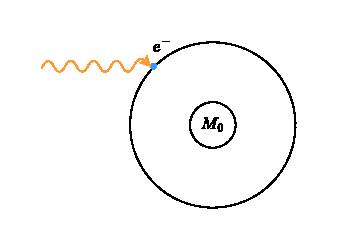
\includegraphics[width=0.6\textwidth]{res/svg/photon_absorbtion.drawio}
\end{figure}
A photon hits an electron moving inside an atom. After the impact the photon is completely absorbed by the electron, which gains speed. We want to find the new speed of the electron. The data of the problem is:
\begin{itemize}
  \item $E_\gamma = \qty{1}{\mega\electronvolt}$
  \item $\gamma_e \simeq 1$
  \item $\gamma_n \simeq 1$
\end{itemize}
This means that the velocity of the nucleus and the electron are non-relativistic before the impact. At the start the total energy is:
\begin{equation}
  E_i = E_\gamma + m_0c^2 + M_0c^2
\end{equation}
After the impact we have:
\begin{equation}
  E_f \simeq m_0\gamma (v) c^2 + M_0c^2
\end{equation}
Here we assume that the recoil speed of the nucleus is negligible with respect to that of the electron given that $M_0 \gg m_0$. Using the conservation of energy we have:
\begin{equation}
  \begin{split}
    &E_i = E_f \\[8pt]
    &E_\gamma + m_0c^2 + \cancel{M_0c^2} = m_0\gamma (v) c^2 + \cancel{M_0c^2} \\[8pt]
    &\gamma (v) = \dfrac{E_\gamma + m_0c^2}{m_0c^2} = 1 + \dfrac{E_\gamma}{m_0c^2} \\[8pt]
  \end{split}
\end{equation}
Since $m_0c^2 \simeq \qty{0.511}{\mega\electronvolt}$ we have:
\begin{equation}
  \gamma \simeq 3 \implies \dfrac{v^2}{c^2} = \dfrac{8}{9} \implies v \simeq 0.94c
\end{equation}
\subsection{Ex.2}
\begin{figure}[H]
  \centering
  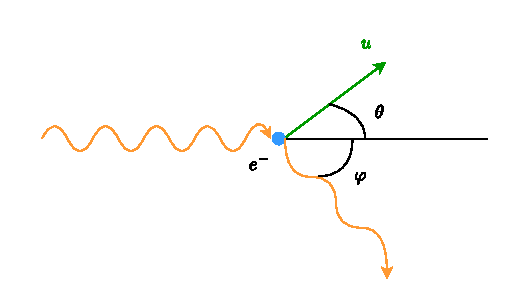
\includegraphics[width=0.6\textwidth]{res/svg/compton_effect.drawio}
\end{figure}
A photon with wavelenght $\lambda_1$ hits an electron at rest. Both the electron and the photon get recoiled in different directions with angle $\theta$ for the electron and $\varphi$ for the photon. This is known as the \textbf{Compton effect}
Because of the conservation of energy the photon must change wavelenght to $\lambda_2$. The energy before the collision is:
\begin{equation}
  E_i = m_0c^2 + h\nu_1
\end{equation}
Instead the energy at the end is:
\begin{equation}
  E_f = m_0\gamma (u) c^2 + h\nu_2
\end{equation}
The momentum instead was:
\begin{equation}
  \vec{P}_i = \begin{pmatrix}
    \dfrac{h\nu_1}{c} \\[8pt]
    0\\[8pt]
    0
  \end{pmatrix}
\end{equation}
And at the end:
\begin{equation}
  \vec{P}_f = \begin{pmatrix}
    \dfrac{h\nu_2}{c}\cos\varphi + m_0u\gamma(u)  \cos\theta \\[8pt]
    -\dfrac{h\nu_2}{c}\sin\varphi + m_0u\gamma(u)  \sin\theta \\[8pt]
    0
  \end{pmatrix}
\end{equation}
Given this we can find that:
\begin{equation}
  \lambda_2 - \lambda_1 = \dfrac{h}{m_0c}\brackets{1-\cos\theta}
\end{equation}
And so this means that $\lambda_2 > \lambda_1$ because the photon loses energy. The quantity $\dfrac{h}{m_0c}$ is called \textbf{Compton wavelenght} $\lambda_c$. In the case of maximum reduction we have $\cos\theta = -1$:
\begin{equation}
  \lambda_2-\lambda_1 = 2\lambda_c
\end{equation}
